\documentclass[
  a4paper,uplatex,dvipdfmx,11pt,
  xcolor = {dvipsnames,svgnames},
  hyperref ={colorlinks=true,citecolor=Navy,linkcolor=NavyBlue,urlcolor=purple}
]{beamer}
\renewcommand{\baselinestretch}{1.4}

% ---refer `texdoc xcolor' at the command line---

% ---Display \subsubsection at the Index
% \setcounter{tocdepth}{3}

% ---Setting about the geometry of the document----
% \usepackage{a4wide}
% \pagestyle{empty}

% ---Physics and Math Packages---
\usepackage{amssymb,amsfonts,amsthm,mathtools}
\usepackage{physics,braket,bm}

% ---underline---
\usepackage{ulem}

% ---cancel---
\usepackage{cancel}

% --- surround the texts or equations
\usepackage{fancybox,ascmac}

% ---settings of theorem environment---
% \usepackage{amsthm}
% \theoremstyle{definition}

% ---settings of proof environment---
% \renewcommand{\proofname}{\textbf{証明}}
% \renewcommand{\qedsymbol}{$\blacksquare$}

% ---Ignore the Warnings---
\usepackage{silence}
\WarningFilter{latexfont}{Some font shapes,Font shape}
\ExplSyntaxOn
\msg_redirect_name:nnn{hooks}{generic-deprecated}{none}
\ExplSyntaxOff

% ---Insert the figure (If insert the `draft' at the option, the process becomes faster.)---
\usepackage{graphicx}
% \usepackage{subcaption}

% ----Add a link to a text---
\usepackage{url,hyperref}
\usepackage{xcolor}
\usepackage{pxjahyper}

% ---Tikz---
\usepackage{tikz,pgf,pgfplots,circuitikz}
\pgfplotsset{compat=1.15}
\usetikzlibrary{intersections,arrows.meta,angles,calc,3d,decorations.pathmorphing,positioning}

% ---Add the section number to the equation, figure, and table number---
\makeatletter
   \renewcommand{\theequation}{\thesection.\arabic{equation}}
   \@addtoreset{equation}{section}
   
   \renewcommand{\thefigure}{\thesection.\arabic{figure}}
   \@addtoreset{figure}{section}
   
   \renewcommand{\thetable}{\thesection.\arabic{table}}
   \@addtoreset{table}{section}
\makeatother

% ---enumerate---
% \renewcommand{\labelenumi}{$\arabic{enumi}.$}
% \renewcommand{\labelenumii}{$(\arabic{enumii})$}

% ---beamer settings---
\usefonttheme{professionalfonts}
\usecolortheme{seahorse}
\setbeamercolor{structure}{fg=white}
\setbeamercolor{local structure}{fg=red}
\setbeamertemplate{itemize item}[ball]
\setbeamertemplate{enumerate item}[circle]
\setbeamercolor{bibliography entry author}{fg=black}
\setbeamercolor{bibliography item}{fg=black}
\setbeamercolor{alerted text}{fg=RoyalBlue}
\setbeamertemplate{frametitle continuation}{}
\setbeamertemplate{footline}[frame number]
\setbeamertemplate{navigation symbols}{} 

% ---tcolorbox---
\usepackage{tcolorbox}
\tcbuselibrary{raster,skins,theorems}
\newtcolorbox{bluebox}[2][]{enhanced,
colframe=RoyalBlue!40!white,
colback=RoyalBlue!10!white,
coltitle=black,
drop fuzzy shadow, title={#2}
,#1}
\newtcolorbox{blueboxblank}[1][]{enhanced,
colframe=RoyalBlue!40!white,
colback=RoyalBlue!10!white,
coltitle=black,
drop fuzzy shadow
,#1}
\newtcolorbox{redbox}[2][]{enhanced,
colframe=DarkRed!40!white,
colback=DarkRed!10!white,
coltitle=black,
drop fuzzy shadow, title={#2}
,#1}

% ---fonts---
\usefonttheme{default}
\renewcommand{\familydefault}{\sfdefault}
\renewcommand{\kanjifamilydefault}{\gtdefault}
\mathversion{bold}
% \usepackage{newtxmath}

% ---citation---
\usepackage{usebib}
\newbibfield{author} 
\newbibfield{year} 
\newbibfield{journal} 
\newbibfield{doi} 
\bibinput{hoge}

\makeatletter
\newcommand*{\journal}{\begingroup\@makeother\#\@mylink}
\newcommand*{\@mylink}[1]{\href{http://dx.doi.org/\usebibentry{#1}{doi}}{\usebibentry{#1}{journal}}\endgroup} 
\makeatother

\newcommand*{\citefone}[2]{
  \begin{tikzpicture}[remember picture, overlay]
    \node[anchor=north east, align=left] at ($(current page.north east)-(0,0.0)$){
    {\tiny
      \cite{#1}
      #2,
      \journal{#1}
      (\usebibentry{#1}{year}).
    }
    };
  \end{tikzpicture}
}

\newcommand*{\citeftwo}[4]{
  \begin{tikzpicture}[remember picture, overlay]
    \node[anchor=north east, align=left] at ($(current page.north east)-(0,0.0)$){
    {\tiny
      \cite{#1}
      #2,
      \journal{#1}
      (\usebibentry{#1}{year}).
    }
    \\[-2.4ex]
    {\tiny
      \cite{#3}
      #4,
      \journal{#3}
      (\usebibentry{#3}{year}).
    }
    };
  \end{tikzpicture}
}

\newcommand*{\citefthree}[6]{
  \begin{tikzpicture}[remember picture, overlay]
    \node[anchor=north east, align=left] at ($(current page.north east)-(0,0.0)$){
    {\tiny
      \cite{#1}
      #2,
      \journal{#1}
      (\usebibentry{#1}{year}).
    }
    \\[-2.4ex]
    {\tiny
      \cite{#3}
      #4,
      \journal{#3}
      (\usebibentry{#3}{year}).
    }
    \\[-2.4ex]
    {\tiny
      \cite{#5}
      #6,
      \journal{#5}
      (\usebibentry{#5}{year}).
    }
    };
  \end{tikzpicture}
}

\newcommand*{\citefonev}[3]{
  \begin{tikzpicture}[remember picture, overlay]
    \node[anchor=north east, align=left, text width=#3cm] at ($(current page.north east)-(0,0.0)$){
    {{\fontsize{5pt}{0pt}\selectfont
      \cite{#1}
      #2,
      \journal{#1}
      (\usebibentry{#1}{year}).\par}
    }
    };
  \end{tikzpicture}
}

\newcommand*{\citeftwov}[5]{
  \begin{tikzpicture}[remember picture, overlay]
    \node[anchor=north east, align=left, text width=#5cm] at ($(current page.north east)-(0,0.0)$){
    {{\fontsize{5pt}{0pt}\selectfont
      \cite{#1}
      #2,
      \journal{#1}
      (\usebibentry{#1}{year}).\par}

      {\fontsize{5pt}{0pt}\selectfont
      \cite{#3}
      #4,
      \journal{#3}
      (\usebibentry{#3}{year}).\par}
    }
    };
  \end{tikzpicture}
}

\newcommand*{\citefthreev}[7]{
  \begin{tikzpicture}[remember picture, overlay]
    \node[anchor=north east, align=left, text width=#7cm] at ($(current page.north east)-(0,0.0)$){
    {{\fontsize{5pt}{0pt}\selectfont
    \cite{#1}
    #2,
    \journal{#1}
    (\usebibentry{#1}{year}).\par}

    {\fontsize{5pt}{0pt}\selectfont
    \cite{#3}
    #4,
    \journal{#3}
    (\usebibentry{#3}{year}).\par}

    {\fontsize{5pt}{0pt}\selectfont
    \cite{#5}
    #6,
    \journal{#5}
    (\usebibentry{#5}{year}).\par}
    }
    };
  \end{tikzpicture}
}


% ---Title---
\title{
  卒業研究
  \texorpdfstring{\\}{}
  \texorpdfstring{\vspace*{5pt}}{}
  {\LARGE
    磁化トーラス上にコンパクト化した
    \\
    超対称模型におけるモジュライ固定
  }
}
\author{
  安倍研究室 \ B4
  \texorpdfstring{\\}{}
  \texorpdfstring{\vspace*{3pt}}{}
  宮根 一樹
}
\date{2024年3月1日(金)}


\begin{document}

\begin{frame}
  \titlepage
\end{frame}


\section{イントロダクション}

\begin{frame}[plain]
  \frametitle{\ }
  \huge \secname
\end{frame}

\begin{frame}
  世の中の物質は細かく見ていくことが可能。

  実験的には「素粒子」が今のところ最小の構成要素。

  \begin{center}
    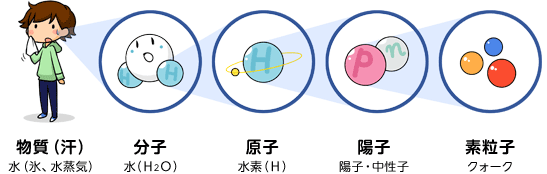
\includegraphics[width=0.8\textwidth]{fig/ILCproject.png}       

    \vspace*{-5pt}
    { \small
      \hspace*{6cm}
      [\href{https://aaa-sentan.org/ILC/about_physics/anatomy01.html}{ILC PROJECT}]
    }   
  \end{center}

\end{frame}

\begin{frame}
  
  \begin{center}

    実験で観測されているのはこの17個の素粒子。
  
    (2012年にヒッグス粒子が発見)

    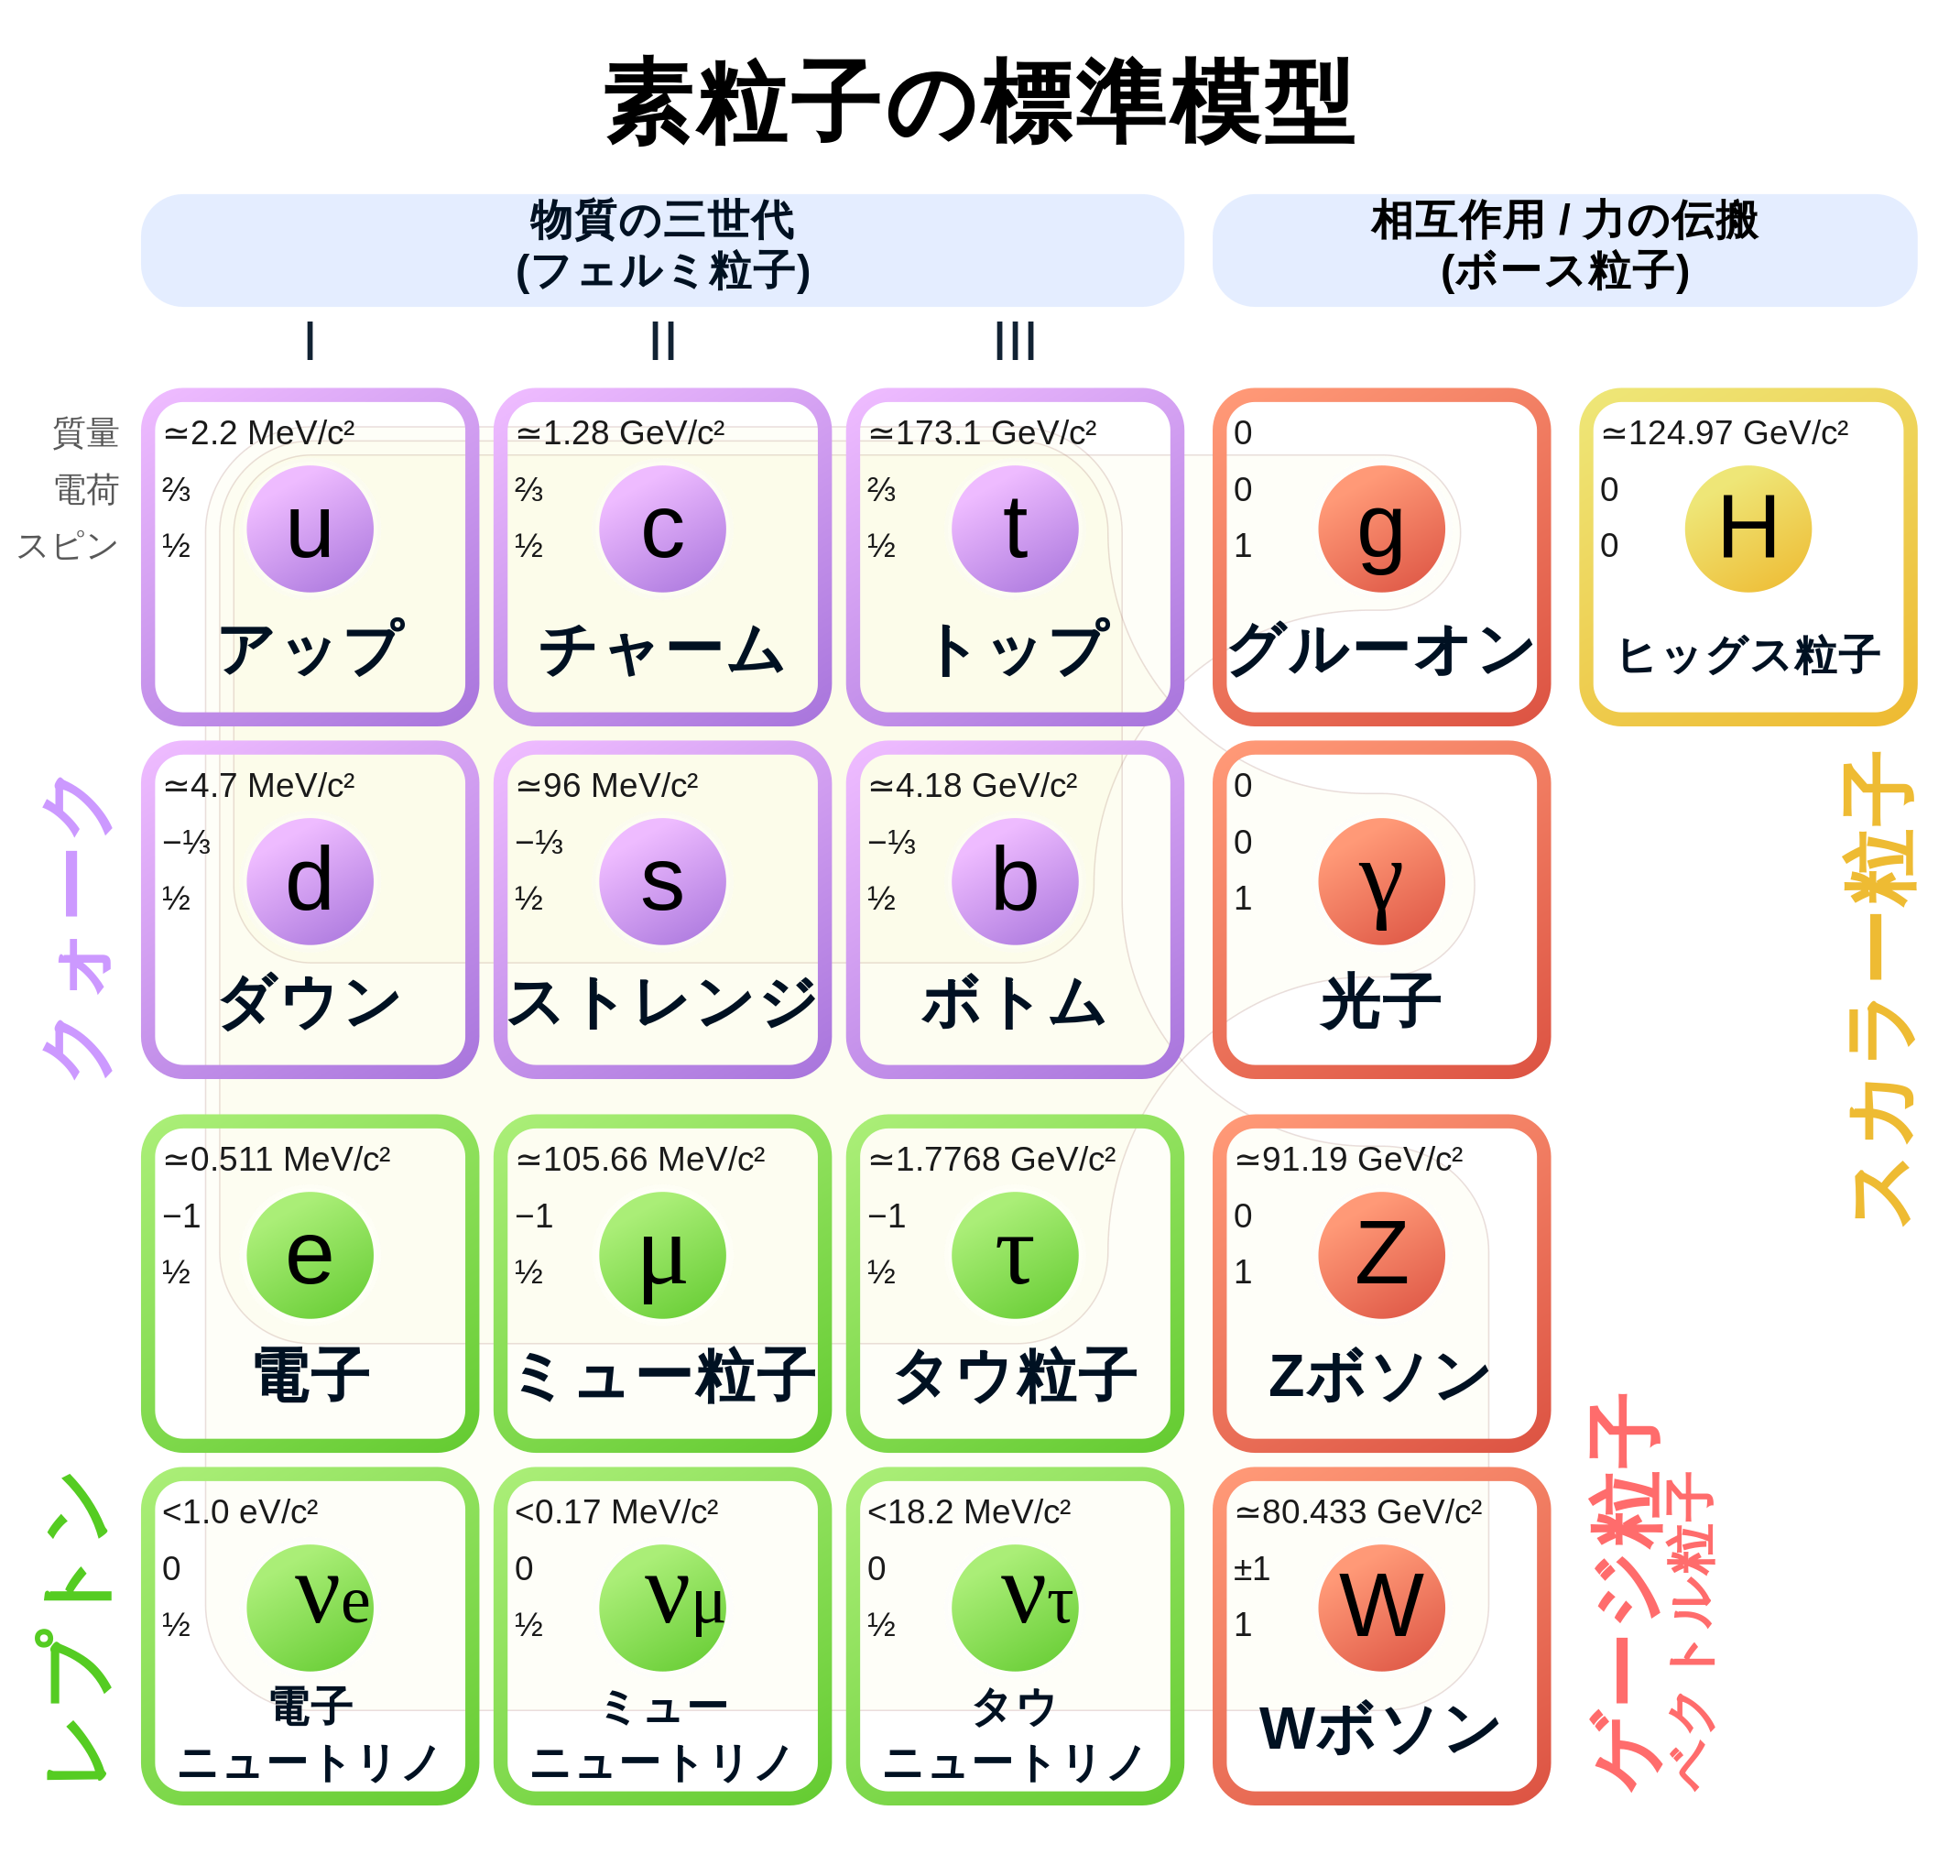
\includegraphics[width=0.6\textwidth]{fig/SM.png}  

    \vspace*{-15pt}
    { \small
      \hspace*{4cm}
      [\href{https://ja.wikipedia.org/wiki/標準模型}{Wikipedia}]
    }
  \end{center}

\end{frame}

\begin{frame}

  この標準模型には、まだ未解決な問題が多数ある。
  
  そもそもどうしてこのような構造をしているのか?

  \begin{itemize}
    \item 
    \textcolor{DarkGreen}{なぜ、}\textcolor{DarkBlue}{物質は3世代存在するのか。}
    \item 
    \textcolor{DarkGreen}{なぜ、}\textcolor{DarkRed}{世代が上がるごとに質量が大きく変わるのか。}
  \end{itemize}

  \only<1>{
    \begin{center}
      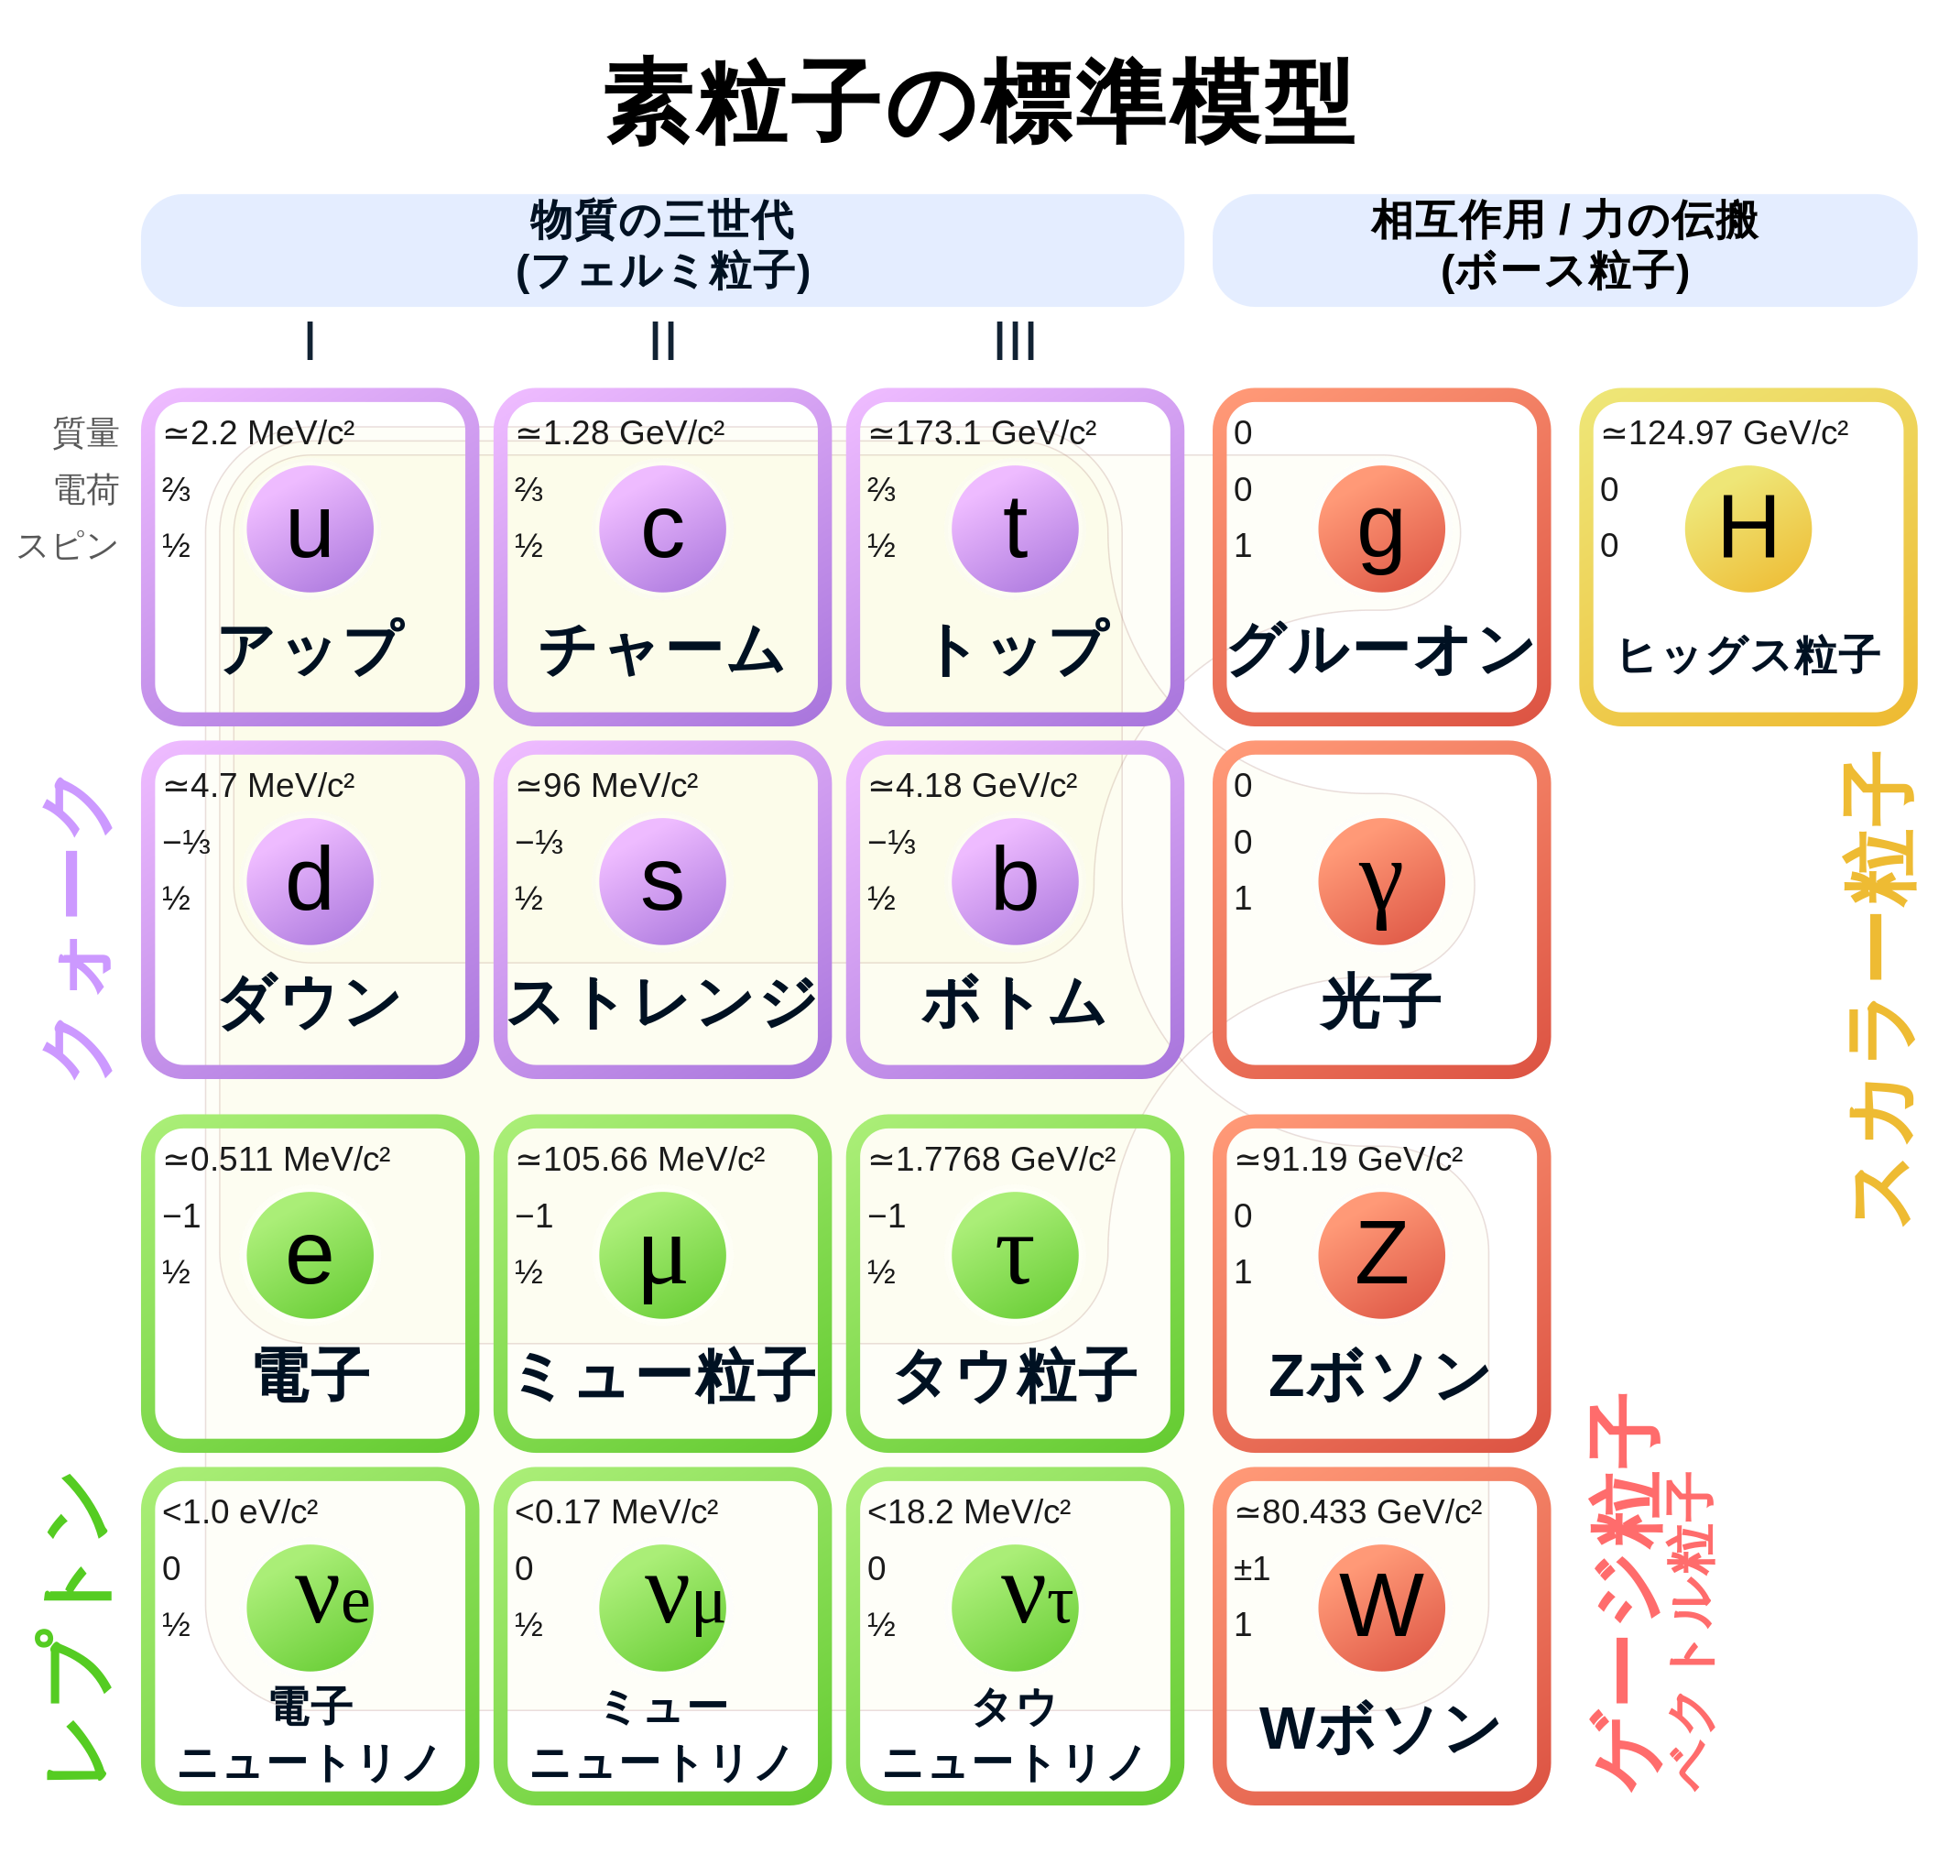
\includegraphics[width=0.5\textwidth]{fig/SM.png}       

      \vspace*{-10pt}
      { \small
        \hspace*{4cm}
        [\href{https://ja.wikipedia.org/wiki/標準模型}{Wikipedia}]
      }   
    \end{center}
  }

  \only<2>{
  \vspace*{10pt}

  標準模型では説明することができない現象がある。
  \begin{itemize}
    \item 
    重力の相互作用
    \item 
    ダークマターなどの未知の粒子
  \end{itemize}

  (ここら辺の話題は\href{https://www2.yukawa.kyoto-u.ac.jp/~soken.editorial/sokendenshi/vol33/1/修士論文_素粒子研究_内田.pdf}{こちらのイントロ}が参考になります。)
  }
  
\end{frame}

\begin{frame}

  

  



  

\end{frame}




% --------------------------

\newcounter{Appendix}
\setcounter{Appendix}{\value{framenumber}}
\setcounter{section}{0}
\renewcommand{\thesubsection}{\Alph{subsection}}
\makeatletter
   \renewcommand{\theequation}{\thesubsection.\arabic{equation}}
   \@addtoreset{equation}{section}
   
   \renewcommand{\thefigure}{\thesubsection.\arabic{figure}}
   \@addtoreset{figure}{section}
   
   \renewcommand{\thetable}{\thesubsection.\arabic{table}}
   \@addtoreset{table}{section}
\makeatother

\section{付録}

\begin{frame}[plain]
  \frametitle{\ }
  \huge \secname
\end{frame}

\subsection{シナリオ}

% \begin{frame}[plain]
%   \frametitle{\thesubsection\ \subsecname}







  
% \end{frame}

% --------------------------

\section{参考文献}
\begin{frame}[plain,allowframebreaks]
  \frametitle{\secname}
  \scriptsize
  \beamertemplatetextbibitems
  \bibliographystyle{ytphys}
  \bibliography{hoge}

  \nocite{Wess_SupersymmetrySupergravity_1992}

\end{frame}


\setcounter{framenumber}{\value{Appendix}}
\end{document}
